\documentclass[11pt,letterpaper]{article}
\usepackage[utf8]{inputenc}



\usepackage{graphicx, geometry, amsmath, amssymb, url, natbib, booktabs, xcolor, listings}
\usepackage{enumitem}
\usepackage{hyperref}
\geometry{margin=1in}
\hypersetup{colorlinks=true, linkcolor=black, citecolor=black, urlcolor=black}
\usepackage{xurl}
\usepackage{caption}
\captionsetup{skip=6pt}
\setlist{itemsep=2pt,topsep=4pt}
\renewcommand{\topfraction}{0.9}
\renewcommand{\bottomfraction}{0.8}
\renewcommand{\textfraction}{0.1}
\renewcommand{\floatpagefraction}{0.8}
\setcounter{topnumber}{3}
\setcounter{bottomnumber}{2}
\setcounter{totalnumber}{5}

\DeclareUnicodeCharacter{2200}{\ensuremath{\forall}}
\DeclareUnicodeCharacter{2203}{\ensuremath{\exists}}
\DeclareUnicodeCharacter{2228}{\ensuremath{\vee}}
\DeclareUnicodeCharacter{2227}{\ensuremath{\wedge}}
\newcommand{\fe}{$\forall$/$\exists$}
\newcommand{\hd}[1]{\begin{tabular}[b]{@{}c@{}}#1\end{tabular}}
\newcommand{\EQ}{\textsc{equiv}}

\title{\vspace{-1.5cm}Peer Agreement as a Reference-Free Signal of NL$\rightarrow$FOL Faithfulness, and Where It Fails}
\author{\vspace{-1cm}}
\date{\vspace{-1cm}}

\begin{document}
\maketitle

\begin{abstract}
Evaluating translations of natural language into first-order logic (FOL) without a gold formula is hard: correct formulas are not unique, benchmark gold is often wrong, and LLM judges reward conventional vocabulary. We ask whether agreement among several systems' formalizations of the same sentence, checked by an SMT solver under a vocabulary alignment that never reads predicate names, measures faithfulness to the text. We freeze a peer agreement score weighted by system reliability on 700 development sentences and evaluate it on 450 fresh sentences from MALLS, FOLIO and ProverQA, formalized by nine current LLMs and labelled twice: by a blinded LLM panel and by solver equivalence to audited gold. Peer agreement reaches 0.827 AUROC on panel labels and 0.874 on solver labels, against 0.791 and 0.727 for a gemini-2.5-flash judge. It is invariant to predicate renaming and flags wrong benchmark gold. The evidence for a practical gain is preliminary. Added to a baseline of judge, roundtrip and structural scores, the score gains about 0.03 AUROC on panel labels with an interval that touches zero, and it does not beat an existing Dawid--Skene agreement estimator. It falls below chance on sentences where most systems share an error, which leaves it far behind the judge on long legal definitions. Directional entailment features and error typing added nothing, and two alternatives based on formal structure, a monotonicity signature and judgment worlds built by a solver, did not beat the judge on current systems. Agreement across systems is a complement, invariant to vocabulary, to a judge that reads the text on short sentences, not a replacement for one.
\end{abstract}

%======================================================================
\section{Introduction}
\label{sec:intro}

Large language models (LLMs) are now the usual semantic parser in pipelines that translate natural-language (NL) text into first-order logic (FOL) and hand the result to a theorem prover or SMT solver \citep{Pan2023,Olausson2023}. Whether such a pipeline reasons correctly depends first on whether each formula says what its sentence says. Measuring that property, which we call \emph{faithfulness}, is the bottleneck. Correct FOL is not unique: two systems can choose different predicate names, split a concept into different predicates, or write logically equivalent formulas, and all of these can be right.

The standard evaluation compares a candidate with a gold formula, by exact match, BLEU overlap or equivalence checked by a prover \citep{Han2022,Yang2023,Thatikonda2025}. This comparison has two known failure modes. The gold itself is often wrong: a recent relabelling study reports incorrect formalizations in roughly 40\% of the entries of the FOLIO validation and MALLS test splits \citep{Brunello2026}. And a candidate can be faithful without being equivalent to the gold, because its vocabulary or granularity differs. Parse rate and structural checks avoid the gold but measure whether formulas are well formed and stable, not what they mean. Reference-free alternatives that read the text, such as LLM-as-a-judge \citep{Zheng2023} and roundtrip verification \citep{Amrollahi2026}, are the natural baselines, but they reward conventional vocabulary and they can share the blind spots of the systems they grade.

A reference-free metric that does not read the text at all has one obvious source of evidence: the other systems. When several independent systems formalize the same sentence, their outputs can be compared with each other by a solver, without any gold and without trusting predicate names. Agreement of this kind is already used to \emph{select} outputs in autoformalization \citep{Li2024,Ryu2024}. Whether it \emph{measures} faithfulness, how much it adds to baselines that read the text, and where it breaks has not been tested on real outputs against labels that do not share its machinery.

We test that question on outputs of nine current LLMs. We score a candidate by the share, weighted by system reliability, of the other systems' formulas that an SMT solver proves logically equivalent to it after a vocabulary alignment that never reads predicate names; we call this the \emph{peer agreement score} and define it in Section~\ref{sec:method}. We freeze its configuration on 700 development sentences and evaluate it on 450 fresh sentences from MALLS, FOLIO and ProverQA, under two independent label families: blinded adjudication by a calibrated panel of three LLMs, and solver equivalence to gold audited by the panel. The evidence supports a complement to a judge, not a replacement, and it is preliminary. Peer agreement is a strong standalone predictor and is exactly invariant to renaming, but its added value over baselines that read the text sits at the edge of statistical significance, it ties an existing latent-class agreement score, and it fails whenever most systems make the same mistake.

\paragraph{Contributions.}
\begin{itemize}
  \item A peer agreement score for NL$\rightarrow$FOL faithfulness that ignores predicate names, weights systems by reliability and was frozen before evaluation (Section~\ref{sec:method}). On 450 fresh sentences it reaches 0.827 AUROC against panel labels and 0.874 against audited solver labels, against 0.791 and 0.727 for a gemini-2.5-flash judge (Section~\ref{sec:main}).
  \item An estimate of what it adds. Stacked on a base of judge, roundtrip and structural scores, it adds $+0.033$ AUROC on panel labels (95\% CI [$-0.001$, 0.066]) and $+0.118$ on solver labels. It does not beat binary Dawid--Skene agreement (0.830), and its components for direction and error typing add nothing (Sections~\ref{sec:increment} and~\ref{sec:ablation}).
  \item A mapped failure boundary. The score is exactly invariant to predicate renaming, where the judge loses 0.151 AUROC on a vocabulary of random tokens (Section~\ref{sec:invariance}). It falls to 0.419 AUROC on sentences whose majority meaning is wrong, and to 0.705 against the judge's 0.927 on long legal definitions (Sections~\ref{sec:sharedbias} and~\ref{sec:complexity}).
  \item A use where agreement is clearly useful: flagging wrong benchmark gold, at 0.837 to 0.859 AUROC and $+0.070$ over a judge run on the gold alone (Section~\ref{sec:gold}).
  \item Negative results for three other reference-free families, a monotonicity signature, judgment worlds built by a solver and instance consequence NLI with a small model, none of which beats the judge on current systems (Section~\ref{sec:otherfamilies}).
\end{itemize}

Figure~\ref{fig:headline} summarizes the finding. Section~\ref{sec:related} places the work, Section~\ref{sec:method} defines the score, Section~\ref{sec:setup} gives the data, labels and protocol, Section~\ref{sec:results} reports results, and Sections~\ref{sec:discussion} to~\ref{sec:conclusion} discuss them, state the limits and conclude.

\begin{figure}[!htbp]
  \centering
  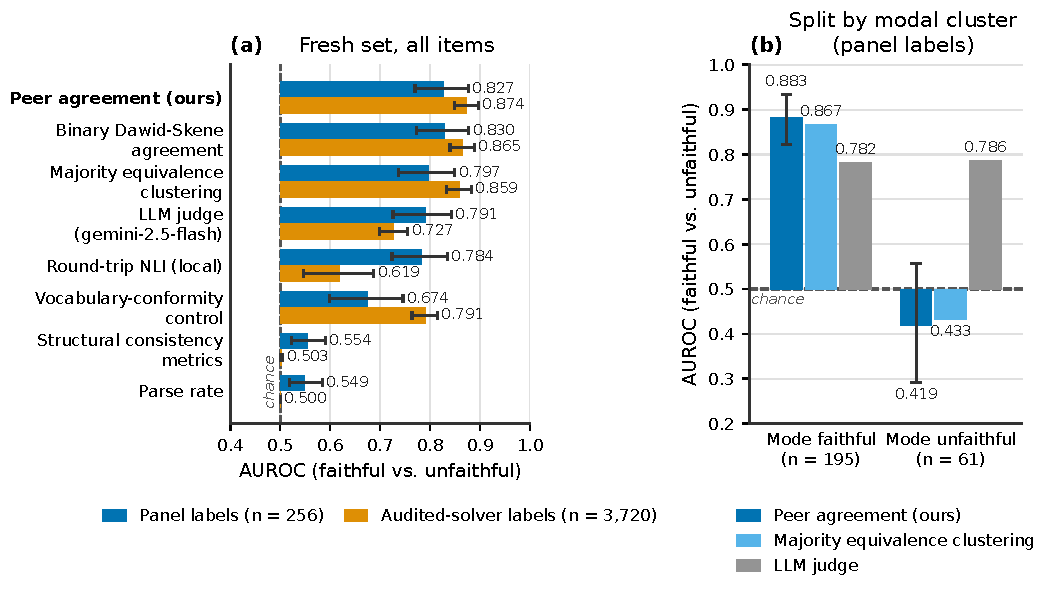
\includegraphics[width=\linewidth,height=0.85\textheight,keepaspectratio]{figures/fig1_v0.pdf}
  \caption{Peer agreement on 450 fresh sentences formalized by nine LLMs. (a) AUROC with 95\% intervals from a bootstrap clustered by sentence, under labels from a blinded LLM panel (256 items) and audited solver labels (3,720 rows; roundtrip NLI on 260 rows). Peer agreement is above the gemini-2.5-flash judge under both label families and ties binary Dawid--Skene agreement; parse rate and the structural consistency metrics are near chance. (b) AUROC under panel labels, split by whether the sentence's modal equivalence cluster is faithful. When most systems share an error, agreement falls below chance while the judge is unaffected.}
  \label{fig:headline}
\end{figure}

%======================================================================
\section{Related Work}
\label{sec:related}

\paragraph{Evaluation against gold and label noise.} FOLIO \citep{Han2022}, MALLS \citep{Yang2023} and ProverQA \citep{Qi2025} supply gold FOL for each sentence and are scored by equivalence or string overlap with the gold. A perturbation study of FOL closeness metrics shows that surface metrics such as BLEU react to text edits more than to operator edits \citep{Thatikonda2025}. For text-to-SQL, test-suite accuracy compares denotations on distinguishing databases \citep{Zhong2020}, and formal verification has exposed errors in that evaluation \citep{Klopfenstein2025}. All of these assume a trustworthy gold. \citet{Brunello2026} relabel FOLIO and MALLS and propose an LLM-assisted framework to direct human reviewers to suspect items; label-error detection with LLM ensembles has also been studied for general NLP benchmarks \citep{Nahum2024}. We use gold only to build labels, audit it with an LLM panel, and use agreement to flag wrong gold, but we do not compare head to head with the relabelling framework.

\paragraph{Reference-free faithfulness.} LLM-as-a-judge \citep{Zheng2023}, roundtrip verification \citep{Amrollahi2026} and scoring of clause conformance \citep{Liu2026} compare a formula, or its back-translation, with the text through a language model. FormalAlign trains an alignment scorer between informal and formal statements \citep{Lu2024}, GenV trains a generative verifier of equivalence to a reference \citep{Singh2026}, and certification that informal and formal statements are equivalent has been proposed for mathematics \citep{Mohammad2026}. Entailment-preserving rates score FOL representations without a reference, but need entailment labels over several premises \citep{Lee2025}. Roundtrip formalization, with equivalence checked by a solver, has been used to evaluate LLMs on truth maintenance without human labels \citep{Karia2024}, and the metrics used for statement autoformalization have themselves been benchmarked against human judgments \citep{Poiroux2024}. Faithfulness of autoformalization in legal reasoning has been examined separately \citep{Wang2026}. Structural probes that need a gold formula, such as the polarity evaluation of SyGNS \citep{Yanaka2021} compare monotonicity marks with a gold formula. These methods all read the text or a reference; our score reads neither, which makes it immune to vocabulary effects and blind to errors the systems share.

\paragraph{Agreement among outputs.} Self-consistency scores agreement within one model's samples \citep{Wang2022}, and semantic entropy clusters sampled generations by bidirectional entailment to estimate uncertainty and detect hallucinations \citep{Kuhn2023,Farquhar2024}. Symbolic-equivalence consistency clusters autoformalizations by solver equivalence and selects from the largest cluster \citep{Li2024}; verification with a SAT solver is used to choose among compositional FOL translations \citep{Ryu2024}; measures based on grammars quantify uncertainty over formal outputs \citep{Ganguly2025}; LINC votes over prover answers \citep{Olausson2023}. Distinguishing inputs judged by an oracle are used to select among programs \citep{Fan2024}. These works use agreement within one model to estimate uncertainty, or agreement among outputs to choose one. We treat agreement across systems as a measurement, compare it with majority clustering in the style of \citet{Li2024}, and report its failure regime.

\paragraph{Estimation without a gold standard.} Latent-class models estimate rater error rates without a gold standard \citep{Dawid1979,Hui1980} and are known to be biased when raters' errors are conditionally dependent \citep{Albert2004}. Benchmarking of LLM judgments without a gold standard has been proposed with a similar logic \citep{Xu2024}. Our reliability weights come from a one-coin Dawid--Skene model, that is, one with a single accuracy parameter per rater, and our result on shared error is the failure under conditional dependence known in this literature, measured directly for NL$\rightarrow$FOL.

%======================================================================
\section{Method}
\label{sec:method}

\subsection{Problem setup}

The input is a sentence $s$ and a candidate formula $F$ from one system, together with peer formulas $P_1, \dots, P_m$: the outputs of $m$ other systems for the same sentence. There is no gold formula and no shared vocabulary; each system names its own predicates. The output is a score in $[0, 1]$ that should be high when $F$ is faithful to $s$. The score may read the peers but never the text, the gold or predicate names.

\subsection{Alignment without predicate names, and pairwise relations}

Two formulas written by different systems use different symbols. For a candidate $F$ and a peer $P$, we search for a map from the predicates and constants of $P$ into those of $F$ that makes the two formulas comparable, using structure only. The search has two levels, tried in order.
\begin{enumerate}
  \item \emph{Bijection}: a bijection of all predicates and constants that preserves arity.
  \item \emph{Partial map}: an injective map that leaves some predicates of $P$ unmatched, as fresh predicates, provided at least 50\% of the predicate occurrences of $P$ are mapped. This level admits peers that decompose a concept differently.
\end{enumerate}

Under each candidate map, the solver decides the relation of $F$ to the mapped peer $P'$. Pairs are first compared by their truth values on 64 fixed random finite structures of domain size 2 and 3, which refutes equivalence soundly and cheaply. Undecided pairs go to an unbounded query, over an uninterpreted sort, to the SMT solver of \citet{Moura2008}, and then to grounding over domains up to size 3. The relation is one of \EQ, \textsc{stronger}, \textsc{weaker}, \textsc{incomparable}, \textsc{contradictory} or \textsc{unalignable} (no admissible map). The search stops at the first map that yields \EQ. Maps never consult predicate names, so the result is unchanged by any consistent renaming.

\subsection{Peer agreement weighted by reliability}

Within a sentence, \EQ{} links the parseable outputs into equivalence clusters. A one-coin Dawid--Skene model \citep{Dawid1979}, that is, one with a single accuracy parameter per system, is fitted over these clusters across all sentences, without labels, and returns one reliability weight $w_j$ per system, floored at 0.05. The \emph{peer agreement score} of $F$ is
\begin{equation}
  \mathrm{PA}(F) = \frac{\sum_{j} w_j \,\mathbf{1}[\mathrm{rel}(F, P_j) = \textsc{equiv}]}{\sum_{j} w_j},
\end{equation}
where the sum runs over the covered peers, including \textsc{unalignable} ones in the denominator. An unparseable candidate, or one with fewer than two covered peers, receives 0.5 and stays in every evaluation. We use the term \emph{modal cluster} for the equivalence cluster that carries the most peer weight for a sentence. Figure~\ref{fig:method} shows the computation.

The configuration was chosen on the 700 development sentences before any fresh label existed, from a 12-configuration grid, by maximizing the mean of panel and solver AUROC, with ties within 0.005 going to the simpler configuration. The frozen configuration uses bijections and partial maps, keeps \textsc{unalignable} peers in the denominator and uses Dawid--Skene weights\footnote{Code: \url{https://github.com/ai-inventor-papers/ai-invention-abf543-do-sentence-and-formula-generalize-the/tree/fork/run_TGmg0LeEY5Gp/round-2/experiment-3}}. Two further components were evaluated and are not part of the score (Section~\ref{sec:ablation}): \emph{granularity definitions}, which let one predicate stand for a conjunction of at most two literals of the other formula, and a \emph{strength profile}, the net weight of peers that are strictly stronger or weaker than $F$, intended to name the error type.

\begin{figure}[!htbp]
  \centering
  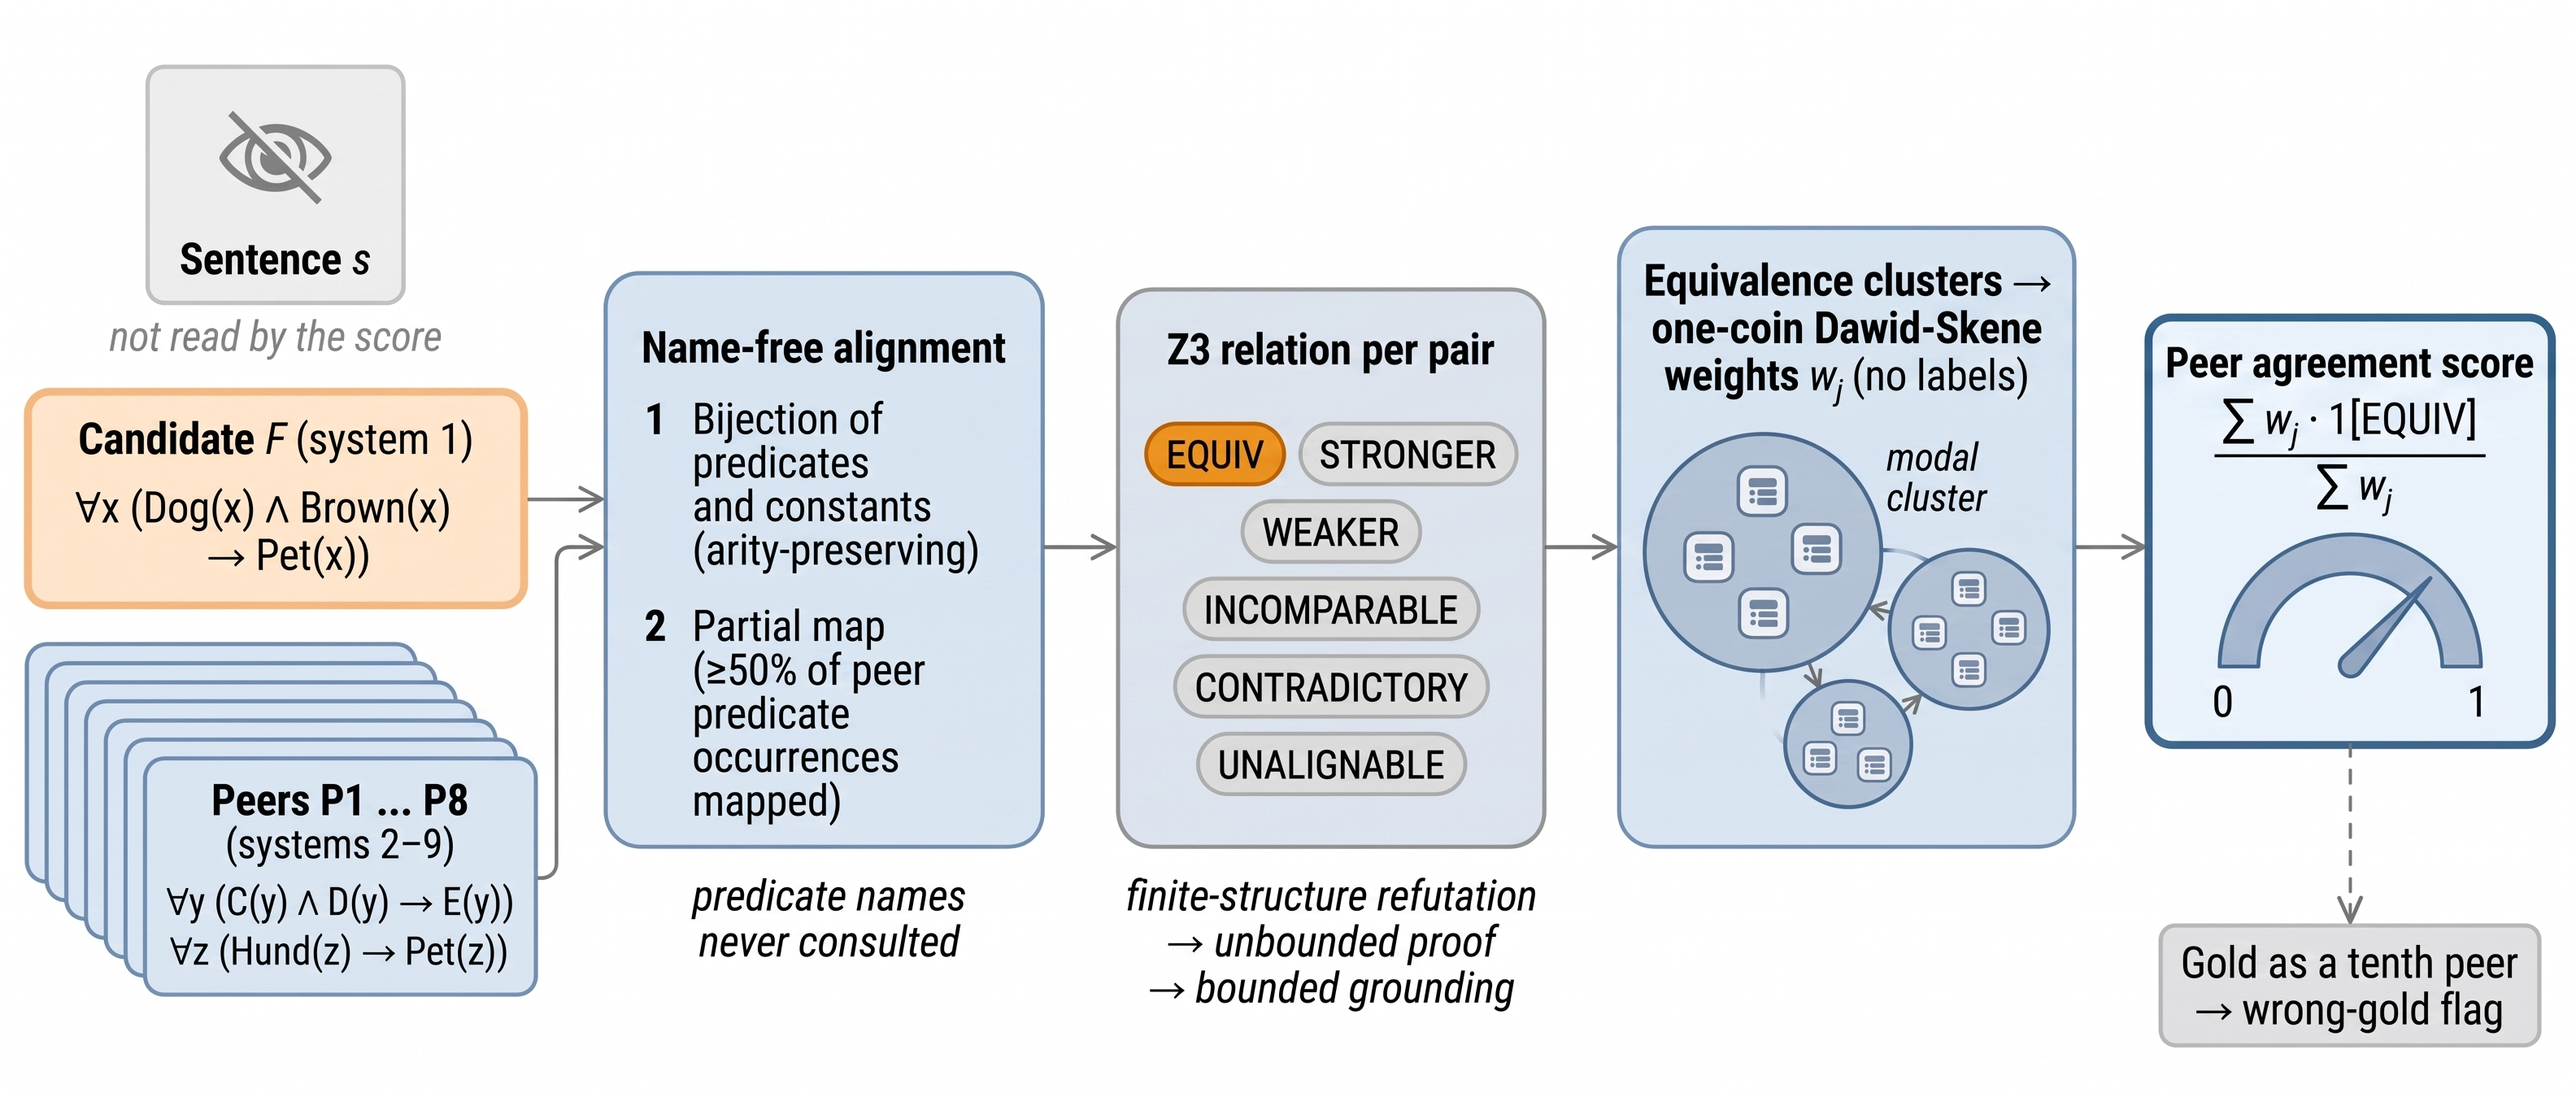
\includegraphics[width=\linewidth,height=0.85\textheight,keepaspectratio]{figures/fig2_v0.jpg}
  \caption{The peer agreement score. A candidate formula is compared with each peer formula (other systems' outputs for the same sentence) after a vocabulary alignment that ignores predicate names (a bijection, then a partial map). An SMT solver decides the logical relation of each aligned pair. EQUIV relations define equivalence clusters, from which a Dawid--Skene model with one accuracy parameter per system, fitted without labels, estimates one reliability weight per system. The score is the weighted share of peers that are equivalent to the candidate. The sentence text and predicate names are never read.}
  \label{fig:method}
\end{figure}

\subsection{Flagging wrong gold}

The same machinery scores a benchmark's shipped gold formula: treat the gold as a tenth system, compute its agreement with the nine system outputs, and flag gold with low agreement. This use needs no extra model call.

%======================================================================
\section{Experimental Setup}
\label{sec:setup}

\subsection{Systems and sentences}

Nine LLMs from seven families, that is, llama-3.1-8b, qwen-2.5-7b, mistral-small-3.2-24b, gpt-4.1-mini, gemini-2.5-flash (no thinking), deepseek-v3.1, gemma-3-27b, phi-4 and gpt-oss-120b, formalized every sentence with one zero-shot prompt that let them name predicates freely, at temperature 0. Two systems, gpt-4.1-mini and llama-3.1-8b, also drew five samples at temperature 0.8.

The \emph{development set} holds 700 sentences: 250 from the MALLS v0.1 test split, 250 from stories of the FOLIO v2 training split disjoint from both FOLIO validation versions, and 200 from the medium and hard levels of the ProverQA development split, with 45.1\% in the top complexity tercile\footnote{Code: \url{https://github.com/ai-inventor-papers/ai-invention-abf543-do-sentence-and-formula-generalize-the/tree/fork/run_TGmg0LeEY5Gp/round-1/dataset-1}}. It was used only for configuration and mechanism tests. The \emph{fresh set} holds 450 new sentences from the same pools (MALLS 170, FOLIO v2 training split 150, ProverQA 130), half in the top complexity tercile, with zero string or story overlap with the development set. It yields 4,050 greedy candidates, of which 222 are unparseable and kept. Complexity is a composite of token count, quantifier count, nesting depth and number of conditions.

The \emph{legal set} is the only material rich in exceptions: 158 sentences from Article~3 of the EU AI Act, GDPR Art.~4, DSA Art.~3, DMA Art.~2, Data Act Art.~2 and the SARA clauses from the US tax code, binned by the number of exception and condition markers (\emph{unless}, \emph{except}, \emph{only}, \emph{provided that} and six others) into 0--1 (91 sentences), 2--3 (51) and 4 or more (16)\footnote{Code: \url{https://github.com/ai-inventor-papers/ai-invention-abf543-do-sentence-and-formula-generalize-the/tree/fork/run_TGmg0LeEY5Gp/round-2/experiment-5}}. The nine systems reach a greedy parse rate of 73.3\% there.

\subsection{Labels}

We use two label families and require a result to hold under both.
\begin{itemize}
  \item \textbf{Panel labels.} A panel of three LLMs, that is, claude-haiku-4.5, grok-4.3 and glm-4.6, drawn from model families other than that of the gemini judges, sees the sentence with the gold and the candidate as two unnamed formulas in random order; the label is the majority of the three votes. Each member first had to reach at least 80\% accuracy on 40 items with known labels. On 99 MALLS items with human corrections the panel agreed with the humans at Cohen $\kappa = 0.57$. We label 609 development items and 256 fresh items weighted to match the sampling strata (fresh Kish effective sample size 202).
  \item \textbf{Audited solver labels} (\emph{solver labels} for short). The panel first audits each shipped gold. A candidate is faithful if the SMT solver proves it equivalent to the audited gold under a bijection of predicates and constants that preserves arity, searched without lexical information. This gives 3,720 labelled fresh rows.
\end{itemize}

The two families have complementary weaknesses. Solver labels share the equivalence checker with the score, so they can favour it; panel labels are LLM judgments, so they can favour LLM judges. Table~\ref{tab:labels} shows why neither alone is enough: shipped gold is wrong on 44\% to 62\% of FOLIO and MALLS items, and about 44\% of candidates that the solver calls not equivalent to audited gold are judged faithful.

\begin{table}[!htbp]
  \centering
  \small
  \caption{Label quality. Wrong-gold rates are the panel's audit of shipped gold; the fourth row is the share judged faithful by the panel among candidates that the solver calls not equivalent to audited gold.}
  \label{tab:labels}
  \begin{tabular}{lcc}
    \toprule
    Quantity & Development (700 sentences) & Fresh (450 sentences) \\
    \midrule
    wrong shipped gold, MALLS & 0.456 & 0.553 \\
    wrong shipped gold, FOLIO v2 training split & 0.620 & 0.620 \\
    wrong shipped gold, ProverQA & 0.175 & 0.146 \\
    judged faithful, not solver equivalent & 0.439 [0.395, 0.486] & 0.438 \\
    agreement of solver and panel & 0.676 & 0.689 \\
    \bottomrule
  \end{tabular}
\end{table}

Among development candidates the panel judged unfaithful, the most frequent primary errors were added conditions (24.9\%), \fe{} choice (21.8\%), dropped conditions (14.4\%) and implication direction or ``only'' (8.4\%); quantifier scope and cardinality together made up about 7\%.

The legal set has no gold, so the same panel judged each candidate from the sentence alone. It labelled 655 sampled candidates, of which 67 were faithful (weighted share 9.4\%), with Fleiss $\kappa = 0.38$ overall and 0.17 on sentences with four or more markers.

\subsection{Baselines}
\label{sec:baselines}

\begin{itemize}
  \item \emph{LLM judge}: gemini-2.5-flash \citep{Comanici2025}, thinking off, temperature 0, asked for the probability that the formula is faithful to the sentence. The \emph{frontier judge} is gemini-2.5-pro with the same prompt.
  \item \emph{Roundtrip}: back-translation of the formula to English, compared with the sentence by NLI with DeBERTa-v3 \citep{He2021} or by the cosine similarity of MiniLM \citep{Wang2020} sentence embeddings \citep{Reimers2019}. On the fresh and legal sets the back-translation used a local Qwen3-8B model \citep{Yang2025}; rows computed this way are marked (L).
  \item \emph{Structural consistency metrics} (\emph{structural metrics} for short): joint loadability, arity consistency within a formula and within a document, and undefined predicates, the stability checks common in NL$\rightarrow$FOL pilots; and \emph{parse rate}.
  \item \emph{Self-consistency}: agreement of a candidate with the same system's samples \citep{Wang2022}.
  \item \emph{Agreement neighbours}: \emph{majority equivalence clustering} (\emph{majority clustering} for short), the share of other outputs in the candidate's cluster of outputs equivalent under a bijection \citep{Li2024}; the posterior of the one-coin model, that is, the probability that the candidate's cluster is the correct one; and \emph{binary Dawid--Skene agreement}, a Dawid--Skene posterior with two classes over the same clusters \citep{Dawid1979}.
  \item \emph{Vocabulary conformity control}: the mean of the Jaccard overlap of predicate names with the peers and the agreement of arity profiles with the peers. It tests whether agreement merely rewards conventional names.
  \item \emph{Error typing judge}: gemini-2.5-flash shown the sentence and the candidate and asked to name one error type from the panel's taxonomy (a local Qwen3-8B substitute on the fresh set).
\end{itemize}

We also evaluated three other reference-free families, which read the text through formal structure (Section~\ref{sec:otherfamilies}). The \emph{monotonicity signature} records, for each concept of the sentence, whether the sentence stays true when the concept is generalized (upward monotone) or specialized (downward monotone). It reads these labels from the text with a rule-based polarity marker \citep{Chen2021} or an LLM substitution probe validated on MED \citep{Yanaka2019}, computes the same labels for the formula exactly with a solver, and scores their agreement. We call the second family \emph{judgment worlds}, an adaptation of the truth value judgment task: a solver builds small worlds that separate a candidate from its own mutants, and an LLM judges only whether the sentence is true in each world, following the idea of distinguishing inputs in \citet{Fan2024}. \emph{Instance consequence NLI} checks ground consequences derived by a prover against the sentence with DeBERTa-v3 NLI \citep{He2021}.

\subsection{Protocol}

The primary measure is the AUROC of each score at the item level against each label family, with 2,000-draw bootstrap intervals clustered by sentence. \emph{Incremental AUROC} is the gain in AUROC, computed on held-out folds, when a score is added to a logistic regression fitted by cross-validation over a fixed base, with folds grouped by sentence. The \emph{base} is [LLM judge, parse rate, roundtrip NLI, roundtrip cosine, structural metrics]. The tests, fixed before the fresh labels existed, were: an increment over the base; a win over majority clustering, binary Dawid--Skene agreement and the vocabulary conformity control; error-type naming; and scoring a lone output with its own samples as peers.

%======================================================================
\section{Results}
\label{sec:results}

\subsection{Peer agreement predicts faithfulness on fresh sentences}
\label{sec:main}

Table~\ref{tab:main} gives every score on the fresh set. Peer agreement reaches 0.827 AUROC against panel labels and 0.874 against audited solver labels. The LLM judge reaches 0.791 and 0.727. Scored with unparseable outputs set to 0 instead of 0.5, peer agreement reaches 0.853 on panel labels. Parse rate and the structural metrics are close to chance on both label families, and the configuration transferred from development (0.777 panel, 0.855 solver) without loss. The three latent-class agreement estimators score within 0.01 of peer agreement on panel labels and 0.009 to 0.024 below it on solver labels. Figure~\ref{fig:headline}a plots the main rows.

\begin{table}[!htbp]
  \centering
  \small
  \caption{AUROC [95\% CI] on the fresh set under panel labels (256 adjudicated items) and audited solver labels (3,720 rows unless stated). (L) marks a baseline computed with a local Qwen3-8B model. Coverage is the share of rows a score covers without the 0.5 default; the two rows that use samples are computed only for gpt-4.1-mini and llama-3.1-8b.}
  \label{tab:main}
  \resizebox{\linewidth}{!}{%
  \begin{tabular}{lllc}
    \toprule
    Score & Panel & Solver & Coverage \\
    \midrule
    \textbf{peer agreement (frozen)} & \textbf{0.827} [0.770, 0.877] & \textbf{0.874} [0.849, 0.897] & 0.945 \\
    latent class, one accuracy per system & 0.834 [0.776, 0.885] & 0.850 [0.823, 0.876] & 0.930 \\
    binary Dawid--Skene agreement & 0.830 [0.773, 0.878] & 0.865 [0.840, 0.889] & 0.930 \\
    latent class, two populations (Hui--Walter) & 0.836 [0.778, 0.887] & 0.852 [0.824, 0.877] & 0.930 \\
    majority equivalence clustering & 0.797 [0.737, 0.850] & 0.859 [0.833, 0.883] & 0.930 \\
    self-consistency, 2 sampled systems & 0.843 [0.777, 0.904], $n=143$ & 0.784 [0.753, 0.813], $n=823$ & 0.993 \\
    peer agreement, own samples as peers & 0.842 [0.775, 0.903], $n=143$ & 0.784 [0.754, 0.814], $n=823$ & 0.993 \\
    LLM judge (gemini-2.5-flash) & 0.791 [0.726, 0.843] & 0.727 [0.698, 0.755] & 1.000 \\
    roundtrip NLI (L) & 0.784 [0.724, 0.835] & 0.619 [0.546, 0.687], $n=260$ & 1.000 \\
    roundtrip cosine (L) & 0.752 [0.686, 0.817] & 0.657 [0.587, 0.730], $n=260$ & 1.000 \\
    vocabulary conformity control & 0.674 [0.598, 0.746] & 0.791 [0.764, 0.815] & 0.945 \\
    error typing judge (L) & 0.659 [0.611, 0.710] & 0.593 [0.557, 0.631], $n=260$ & 1.000 \\
    structural consistency metrics & 0.554 [0.522, 0.590] & 0.503 [0.500, 0.505] & 1.000 \\
    parse rate & 0.549 [0.518, 0.584] & 0.500 [0.500, 0.500] & 1.000 \\
    strength profile (directional component) & 0.415 [0.358, 0.467], $n=245$ & 0.464 [0.449, 0.480] & 1.000 \\
    \bottomrule
  \end{tabular}}
\end{table}

Two checks address the simplest artefacts. First, the score does not merely reproduce the solver label: inside the 168 panel items that the solver calls not equivalent to audited gold, where solver labels call every item wrong, peer agreement still separates faithful from unfaithful at 0.776 [0.679, 0.858], against 0.738 for the judge. Second, the score does not merely reward conventional vocabulary: it beats the vocabulary conformity control by $+0.152$ on panel labels and $+0.083$ on solver labels (Table~\ref{tab:tests}). Within a sentence, over 70 pairs of one faithful and one unfaithful output, peer agreement orders the pair correctly 0.929 of the time against 0.786 for the judge; the pairs were sampled as one modal and one minority output per sentence, which is the comparison agreement is built for.

Across nine systems, the ordering of mean scores per system agrees with the faithful rate per system at Kendall $\tau = 0.889$ under solver labels and 0.556 under panel labels; the LLM judge reaches 0.722 and 0.833. With nine systems these correlations are descriptive.

\subsection{The incremental signal is small and ties an existing agreement score}
\label{sec:increment}

Table~\ref{tab:tests} gives the comparisons fixed in advance. Added to the base, peer agreement raises panel AUROC from 0.886 to 0.919, a gain of $+0.033$ whose 95\% confidence interval just includes zero ([$-0.001$, 0.066]); a directional test at the 5\% level gives a lower bound of $+0.005$. Under solver labels the gain is $+0.118$ [0.051, 0.192]. A placebo that shuffles the score within corpus and complexity strata adds $-0.003$. Against a base without the roundtrip features, the gain is $+0.126$ [0.066, 0.189] on panel labels. On the development set the panel increment of latent-class agreement over the same base was of similar size, $+0.019$ [$-0.003$, 0.043]. We therefore read the evidence as an increment of about 0.02 to 0.03 AUROC over a base of judge and roundtrip scores on short sentences, at the edge of significance under panel labels.

\begin{table}[!htbp]
  \centering
  \small
  \caption{Comparisons fixed in advance, on the fresh set. Differences are paired, with 95\% intervals from a bootstrap clustered by sentence.}
  \label{tab:tests}
  \begin{tabular}{lll}
    \toprule
    Comparison & Panel & Solver \\
    \midrule
    base + peer agreement $-$ base & $+0.033$ [$-0.001$, 0.066] & $+0.118$ [0.051, 0.192] \\
    same, placebo (score shuffled within strata) & $-0.003$ [$-0.016$, 0.008] & $-0.001$ [$-0.010$, 0.007] \\
    peer agreement $-$ majority equivalence clustering & $+0.030$ [0.012, 0.049] & $+0.015$ [0.005, 0.026] \\
    peer agreement $-$ binary Dawid--Skene agreement & $-0.003$ [$-0.024$, 0.017] & $+0.009$ [$-0.000$, 0.019] \\
    peer agreement $-$ vocabulary conformity control & $+0.152$ [0.096, 0.209] & $+0.083$ [0.066, 0.102] \\
    \bottomrule
  \end{tabular}
\end{table}

Peer agreement beats majority clustering under both label families, but it does not beat binary Dawid--Skene agreement on panel labels ($-0.003$). The gain over the nearest published mechanism \citep{Li2024} is real but modest, and an existing latent-class estimator already captures it.

\subsection{The reliability weights carry the gain; direction and error typing do not}
\label{sec:ablation}

Table~\ref{tab:ablation} builds the score one component at a time on the fresh set. Agreement under bijections alone, with uniform weights, already reaches 0.801 panel and 0.864 solver AUROC. Partial maps change nothing here, although on the development set they carried the whole gain over agreement under bijections alone (0.636 to 0.763 panel). Granularity definitions lower AUROC. Dawid--Skene weights carry the step to 0.827 and 0.874.

\begin{table}[!htbp]
  \centering
  \small
  \caption{Component ablation on the fresh set, AUROC.}
  \label{tab:ablation}
  \begin{tabular}{lcc}
    \toprule
    Configuration & Panel & Solver \\
    \midrule
    bijection only, uniform weights & 0.801 & 0.864 \\
    \quad + partial maps, uniform weights & 0.801 & 0.863 \\
    \quad + granularity definitions, uniform weights & 0.791 & 0.839 \\
    bijection + partial maps, Dawid--Skene weights (frozen) & \textbf{0.827} & \textbf{0.874} \\
    frozen + granularity definitions & 0.820 & 0.859 \\
    frozen + strength profile (stacked, held-out folds) & 0.791 & 0.867 \\
    strength profile alone & 0.415 & 0.464 \\
    \bottomrule
  \end{tabular}
\end{table}

The directional components failed. The strength profile alone ranks candidates below chance (0.415), and adding it to the score lowers panel AUROC. Error typing from the strength profile named the panel's primary error type for 12.2\% of fresh unfaithful items, against 25.5\% for always answering ``added condition''; on development items the figures were 21.3\% against 25.7\%, and on legal items 4.4\% against 21.9\%. Granularity definitions have a mechanical cost as well. Under constructed truth, a definition of the form $Q := \neg P$ absorbs a single negation (detection 0.511 with definitions, 1.000 without), a definition that adds a conjunct absorbs a dropped restrictor (0.659 against 0.995), and the definitions add 11.9\% spurious equivalences between formulas from unrelated sentences\footnote{Code: \url{https://github.com/ai-inventor-papers/ai-invention-abf543-do-sentence-and-formula-generalize-the/tree/fork/run_TGmg0LeEY5Gp/round-2/experiment-4}}.

Detection per real error type is descriptive at the sizes of the fresh set (10 to 27 errors per class). Peer agreement was strongest on \fe{} errors (0.896) and implication direction (0.881); the judge was strongest on unparseable outputs, negation and quantifier scope.

\subsection{Agreement is exactly invariant to vocabulary}
\label{sec:invariance}

Because alignment never reads names, renaming cannot move the score. We tested this under constructed truth, where labels come from how items were built rather than from any annotator. On 223 development sentences with faithful gold, the gold was rendered in the modal peer's vocabulary, in random tokens and in WordNet synonyms, and the same operator perturbations (negation, added and dropped conjuncts, \fe{}, implication reversal, argument swap) produced 739 \emph{mutants} per rendering: perturbed formulas that are not logically equivalent to the gold. In the \emph{crossed} condition the faithful formula uses random tokens while its mutants use conventional names. Figure~\ref{fig:vocab} shows the result. Peer agreement without granularity definitions separates faithful formulas from mutants at 0.999 AUROC in every rendering. The LLM judge falls from 0.945 with conventional names to 0.794 with random tokens and 0.763 in the crossed condition. The vocabulary conformity control collapses to 0.176 in the crossed condition, as a conformity score must.

\begin{figure}[!htbp]
  \centering
  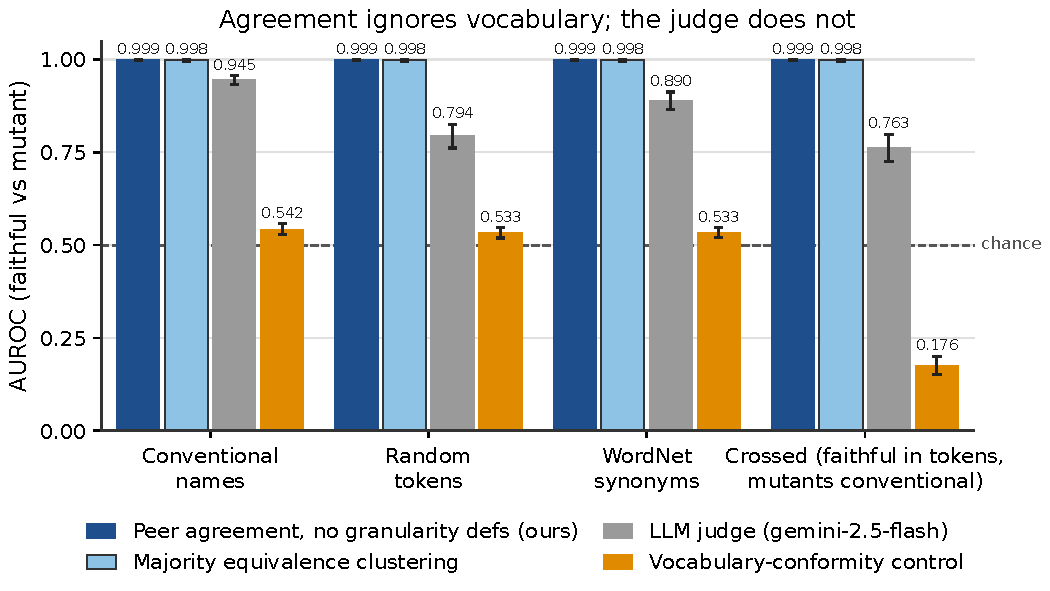
\includegraphics[width=\linewidth,height=0.85\textheight,keepaspectratio]{figures/fig3_v0.pdf}
  \caption{Constructed vocabulary test on 223 development sentences with faithful gold: AUROC of faithful formulas against 739 operator mutants, with the same formulas rendered in the modal peer's vocabulary, in random tokens, in WordNet synonyms, and crossed (faithful formula in random tokens, mutants in conventional names). Peer agreement (without granularity definitions) and majority clustering are unchanged across renderings; the LLM judge loses up to 0.182 AUROC and the vocabulary conformity control collapses in the crossed condition.}
  \label{fig:vocab}
\end{figure}

On real candidates the same holds. Over 1,695 rewrites of 400 fresh candidates that the solver proved equivalent to the original, the false alarm rate, the share of rewrites whose score changed by more than 0.05 or whose modal cluster changed, was 0.25\% for synonym renamings, 0.50\% for random renamings and zero for contrapositive, De Morgan and reorder rewrites. The vocabulary conformity control changed on 86.4\% of synonym renamings. Public benchmarks may have leaked into the training data of LLM judges \citep{Sainz2023}, so we also compared original sentences with renamed versions. On 104 sentences paired with paraphrases whose entities were renamed, the judge's mean score dropped by 0.096 on paraphrases while its AUROC did not change significantly ($-0.022$ [$-0.067$, 0.030]); agreement is invariant to such renaming by construction.

\subsection{Agreement fails when most systems share an error}
\label{sec:sharedbias}

Agreement cannot see a mistake that most peers make. On the fresh set we split panel items by whether the modal cluster of their sentence is faithful. Where it is, peer agreement reaches 0.883 [0.822, 0.934] against the judge's 0.782. Where it is not (61 items), peer agreement falls to 0.419 [0.292, 0.557], below chance, while the judge holds 0.786 (Figure~\ref{fig:headline}b). Majority clustering behaves the same way (0.867 and 0.433). Because the correctness of the modal cluster is read from the labels, this split is descriptive.

A controlled \emph{dose test} isolates the mechanism (Figure~\ref{fig:dose}a). For 200 development sentences, $k$ of the eight peers were replaced by renamed copies of a mutant, over four operators (560 items). For the configuration without granularity definitions, detection, the probability that the faithful formula scores above the mutant, falls from 0.988 at $k = 0$ to 0.791 at $k = 2$, 0.409 at $k = 4$ and 0 at $k = 8$ when peers are replaced in random order, and reaches 0 already at $k = 4$ when faithful peers are replaced first. Renamed copies were recognized as equivalent in 502 of 502 audited pairs, and for the development configuration the observed curve equals the curve predicted from peer weight alone at every $k$. The boundary is therefore arithmetic, not a property of the solver. On real development data (Figure~\ref{fig:dose}b), \emph{concordance within sentences}, that is, the probability that a faithful output scores above an unfaithful output of the same sentence, is 0.831 when clusters with the wrong meaning hold less than a quarter of the peer weight and 0.449 when they hold three quarters or more; the logistic slope is $-2.08$ [$-2.55$, $-1.61$], and the modal cluster is wrong in 284 of 700 sentences.

\begin{figure}[!htbp]
  \centering
  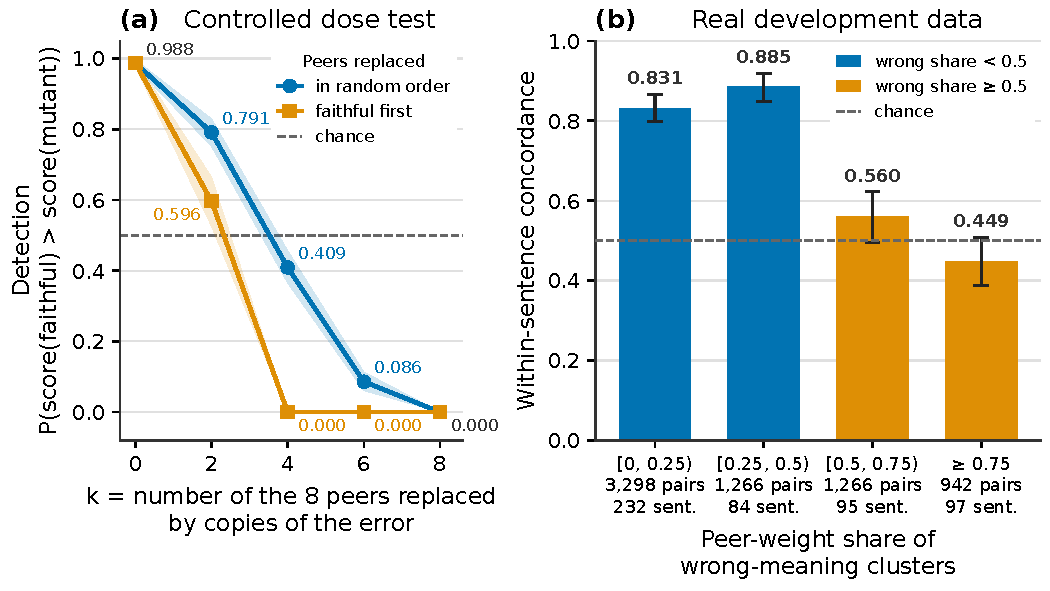
\includegraphics[width=\linewidth,height=0.85\textheight,keepaspectratio]{figures/fig4_v0.pdf}
  \caption{The boundary set by shared error. (a) Controlled dose test on 200 development sentences (560 items, four operators): probability that the faithful formula scores above a mutant when $k$ of its eight peers are replaced by renamed copies of the mutant, for the configuration without granularity definitions, replacing peers in random order or faithful peers first. (b) Real development data (6,772 faithful $\times$ unfaithful pairs in 508 sentences, development configuration): concordance within sentences of the agreement score by the share of peer weight held by clusters with the wrong meaning, with 95\% intervals; logistic slope $-2.08$ [$-2.55$, $-1.61$].}
  \label{fig:dose}
\end{figure}

\subsection{Complexity and long legal definitions}
\label{sec:complexity}

The regime that matters most for practical pipelines is long, heavily conditioned text. On the fresh set, under panel labels, the score's lead over the judge shrinks with complexity: $+0.088$, $+0.107$ and $-0.028$ in the bottom, middle and top terciles (slope $-0.058$ [$-0.135$, 0.022], not significant). Figure~\ref{fig:complexity}a breaks this down by the four complexity features. Peer agreement is weakest on candidates with two or more quantifiers (0.659 against the judge's 0.778), on nesting depth 4--5 and on sentences longer than 20 tokens, and strongest with three or more conditions (0.871 against 0.787). Public corpora are rich in connectives rather than in exceptions: FOLIO contains one \emph{unless} or \emph{except} in 2,656 pairs of sentence and formula.

On the legal set the result is clearly negative for agreement (Table~\ref{tab:legal}, Figure~\ref{fig:complexity}b). Peer agreement reaches 0.705, and 0.672 without granularity definitions; the LLM judge reaches 0.927 and the frontier judge 0.852. The score trails the judge in every marker bin. Stacked on [judge, parse rate] it adds $+0.021$ [$-0.001$, 0.046]; over the full base it adds $+0.008$ [$-0.012$, 0.028]. Equivalence is rare on long text, 4.8\% of legal pairs against 38.5\% on fresh sentences, so the fitted system weights all fell to the 0.05 floor. Shared error dominates: in 76\% of the 62 sentences with a labelled modal cluster, that cluster is unfaithful. Where the modal cluster was unfaithful, the score fell to 0.624 while the judge held 0.946.

\begin{table}[!htbp]
  \centering
  \small
  \caption{Legal set, weighted AUROC against panel labels from the sentence alone (655 items, 67 faithful), by exception and condition marker count.}
  \label{tab:legal}
  \begin{tabular}{lccccc}
    \toprule
    \hd{Marker bin\\(items, faithful)} & \hd{Peer\\agreement} & \hd{LLM\\judge} & \hd{Frontier\\judge} & \hd{Majority\\clustering} & \hd{Roundtrip\\NLI (L)} \\
    \midrule
    all (655, 67) & 0.705 & \textbf{0.927} & 0.852 & 0.754 & 0.694 \\
    \quad 95\% CI & [0.608, 0.792] & [0.900, 0.949] & [0.786, 0.904] & [0.670, 0.828] & [0.601, 0.773] \\
    0--1 markers (419, 56) & 0.726 & \textbf{0.923} & 0.862 & 0.795 & 0.728 \\
    2--3 markers (162, 6) & 0.566 & \textbf{0.931} & 0.823 & 0.548 & 0.534 \\
    $\geq$ 4 markers (74, 5) & 0.685 & \textbf{0.909} & 0.785 & 0.493 & 0.685 \\
    \bottomrule
  \end{tabular}
\end{table}

The legal labels are the weakest in the study. They come from an LLM panel judging the sentence alone, with $\kappa = 0.17$ on the bin with four or more markers and member faithful rates from 0.04 to 0.22, and the panel's sensitivity to exception errors was not certified. The frontier judge scoring 0.075 below the LLM judge (gemini-2.5-flash) against these labels suggests that part of the judges' lead is agreement between LLM judges. The ordering held under the labels of each single panel member and on the 515 unanimous items (peer agreement 0.866, judge 0.974), but with 11 faithful items in the upper two bins these bins do not support a conclusion.

\begin{figure}[!htbp]
  \centering
  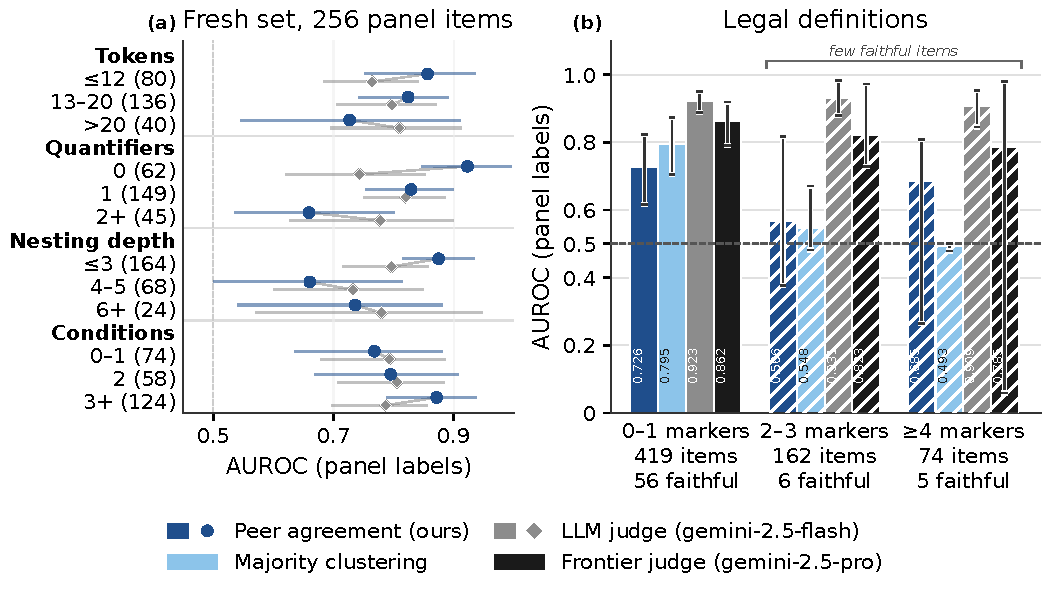
\includegraphics[width=\linewidth,height=0.85\textheight,keepaspectratio]{figures/fig5_v0.pdf}
  \caption{Reliability by complexity under panel labels. (a) Fresh set: AUROC of peer agreement and the LLM judge per stratum of the four complexity features (items per stratum in parentheses); agreement leads on short sentences, sentences without quantifiers, sentences with shallow nesting and sentences with three or more conditions, and trails on two or more quantifiers, deeper nesting and long sentences. (b) Legal definitions (655 items, panel labels from the sentence alone) by number of exception and condition markers: every reference-free score trails both judges in every bin; the upper two bins hold only 6 and 5 faithful items.}
  \label{fig:complexity}
\end{figure}

\subsection{Agreement flags wrong benchmark gold}
\label{sec:gold}

Treating the shipped gold as a tenth peer gives a reference-free flag for wrong gold (Table~\ref{tab:gold}). Against the panel's audit of 700 development golds, of which 43\% are wrong, the flag reaches 0.837 AUROC, and 0.891 on ProverQA, where 19 of the 25 golds it scores lowest are wrong at a 17.5\% base rate. On the 450 fresh golds it reaches 0.859, with precision 0.80 among the 50 golds it scores lowest. The flag complements a judge run on the gold: stacked with it, AUROC rises from 0.825 to 0.896.

\begin{table}[!htbp]
  \centering
  \small
  \caption{Wrong-gold flagging with the gold as a tenth peer, against the panel's gold audit.}
  \label{tab:gold}
  \begin{tabular}{ll}
    \toprule
    Population & AUROC [95\% CI] \\
    \midrule
    development, pooled (700 golds, 43\% wrong) & 0.837 [0.809, 0.864] \\
    development, ProverQA / MALLS / FOLIO & 0.891 / 0.783 / 0.733 \\
    fresh, pooled (450 golds, 46\% wrong) & 0.859 \\
    development: LLM judge on gold $\rightarrow$ + peer agreement & 0.825 $\rightarrow$ 0.896, $+0.070$ [0.045, 0.096] \\
    development: error typing judge on gold $\rightarrow$ + peer agr. & 0.841 $\rightarrow$ 0.889, $+0.048$ [0.028, 0.070] \\
    \bottomrule
  \end{tabular}
\end{table}

\subsection{Other reference-free families do not beat a judge on current systems}
\label{sec:otherfamilies}

Table~\ref{tab:families} reports the three other reference-free families described in Section~\ref{sec:baselines}. On 2023-era Logic-LM outputs for the FOLIO validation split \citep{Pan2023}, labelled by solver equivalence to gold, the signature and the worlds both ranked candidates above an LLM judge\footnote{Code: \url{https://github.com/ai-inventor-papers/ai-invention-abf543-do-sentence-and-formula-generalize-the/tree/fork/run_TGmg0LeEY5Gp/round-1/experiment-1}}\textsuperscript{,}\footnote{Code: \url{https://github.com/ai-inventor-papers/ai-invention-abf543-do-sentence-and-formula-generalize-the/tree/fork/run_TGmg0LeEY5Gp/round-1/experiment-2}}. On current systems the order reversed. The signature's polarity comparison added nothing beyond its own lexical alignment ($+0.011$ [$-0.010$, 0.031]), and it named real error types less often than always answering the majority class (11.1\% against 24.9\%). The worlds, made deterministic and free of false alarms on logical rewrites, lost to the judge in the top complexity tercile by $-0.098$ [$-0.184$, $-0.014$], the regime where they had led on the older screen. The judge that collapsed on the older screen's top tercile (0.552) held 0.772 there on current outputs.

\begin{table}[!htbp]
  \centering
  \small
  \caption{Reference-free families on two populations. The 2023 screen is 835 Logic-LM candidates for 300 sentences of the FOLIO validation split, with solver labels against gold; the current systems are the 609 development panel items from nine current LLMs. Judge values come from runs on the same items as each row; three repeated judge runs on the items of current systems gave 0.762, 0.749 and 0.745.}
  \label{tab:families}
  \begin{tabular}{lcc}
    \toprule
    Score & 2023 screen & Current systems \\
    \midrule
    monotonicity signature, rule-based polarity & 0.718 & 0.642 \\
    monotonicity signature, LLM probe & 0.711 & 0.657 \\
    judgment worlds & 0.701 & 0.665 \\
    instance consequence NLI (DeBERTa) & 0.603 & n/a \\
    latent-class agreement, one accuracy per system & 0.853 & 0.756 \\
    LLM judge (gemini-2.5-flash) & 0.644 to 0.665 & 0.745 to 0.762 \\
    frontier judge (gemini-2.5-pro) & n/a & 0.825 \\
    roundtrip NLI & 0.660 & 0.734 \\
    \bottomrule
  \end{tabular}
\end{table}

Two lessons carry over to the agreement results. A screen on older systems can reverse on current ones, which is why we froze the score on development data and confirmed it on fresh sentences. And the frontier judge's lead depends on the labels: on the same 608 development items it scored 0.827 against panel labels and 0.738 against solver labels, while the LLM judge moved by only $+0.005$, and it scored outputs of its own model family higher (0.853 against 0.817), as LLM evaluators are known to favour their own generations \citep{Panickssery2024}.

%======================================================================
\section{Discussion}
\label{sec:discussion}

The evidence supports a narrow role for agreement across systems. On short benchmark sentences it is at least as predictive as an LLM judge with a fixed prompt under both label families. Adding it to a base of judge and roundtrip scores gains about 0.03 AUROC, with a 95\% confidence interval that touches zero. It also has two properties that metrics reading the text lack: it is exactly invariant to vocabulary, and it can audit the gold itself. Its costs are equally concrete. It needs outputs from several independent systems for the same sentence. When those outputs already exist it costs no API call and about 0.16\,s of solver time per item, but generating eight peers costs about \$0.00039 per short item, 13 times the judge's \$0.00003, and \$0.0019 per legal item, 31 times the judge. With a system's own samples as peers it reduces to sampling self-consistency (0.842 against 0.843 on fresh panel items).

The result on shared error explains most of what agreement cannot do. Every error that most systems make is invisible to it, and the constructed dose curve shows the failure is exact arithmetic of peer weight, the problem of conditional dependence that latent-class estimation has long had in epidemiology \citep{Albert2004}. That regime is common on long legal definitions, where three quarters of modal clusters were unfaithful. Directional machinery did not help: solver-computed strength relations to peers neither ranked candidates nor named errors, even though the four most frequent real errors change logical strength.

Two design choices mattered for credibility. Requiring a result under both panel and audited solver labels separated what agreement tracks from what either label family rewards: the judge looks much stronger under panel labels, agreement under solver labels, and only effects that hold under both are claimed. Freezing on development sentences and confirming on disjoint sentences guarded against the reversal we observed for the monotonicity signature and the judgment worlds between older and current systems.

In practice, the results suggest using agreement as a complement to a judge that reads the text when several systems' outputs are already available, as a check invariant to vocabulary, and as a gold auditor for benchmark curation, but not as a standalone faithfulness metric for long text or text rich in exceptions.

%======================================================================
\section{Limitations}
\label{sec:limitations}

\begin{itemize}
  \item \textbf{Thin increment.} The increment under panel labels over the base of judge and roundtrip scores is $+0.033$ with a 95\% confidence interval of [$-0.001$, 0.066]. It is significant only under a directional test, and it matches, rather than exceeds, what latent-class agreement showed on development data. The fresh panel has 256 items (Kish effective sample size 202).
  \item \textbf{No gain over an existing estimator.} Peer agreement does not beat binary Dawid--Skene agreement on panel labels, and its gain over majority clustering comes from reliability weighting, not from anything new in the comparison.
  \item \textbf{LLM labels.} Panel labels are LLM judgments, with $\kappa = 0.57$ against human corrections on MALLS and 0.37 pairwise agreement on the primary error type. No human adjudication was used. On legal text the labels come from the sentence alone, $\kappa$ falls to 0.17 on sentences with four or more markers, and the panel's sensitivity to exception errors is uncertified; the legal conclusions are correspondingly weak.
  \item \textbf{Substituted and missing baselines.} Roundtrip baselines on the fresh and legal sets used a local Qwen3-8B back-translation, which favoured outputs of Qwen models (0.968 against 0.766 roundtrip NLI AUROC on the 18 panel items generated by Qwen models). The frontier judge was not run on fresh items. GenV \citep{Singh2026}, FormalAlign \citep{Lu2024} and the relabelling framework of \citet{Brunello2026} were not benchmarked.
  \item \textbf{Operating conditions.} The score needs several independent systems per sentence and cannot score a lone output beyond what self-consistency gives. It fails under shared error, which is frequent on long text.
  \item \textbf{Signal between sentences.} On development solver labels, shuffling labels within sentences leaves the score at 0.70 AUROC against a true 0.82, so much of its AUROC at the item level separates easy from hard sentences rather than candidates within a sentence. The fresh comparison within sentences (0.929 against 0.786 for the judge over 70 pairs) used pairs sampled from one modal and one minority output per sentence, a design that favours agreement.
  \item \textbf{Error types.} No reference-free method in the study named real error types better than always predicting the most frequent type.
\end{itemize}

%======================================================================
\section{Conclusion}
\label{sec:conclusion}

Across nine current LLMs and 450 fresh sentences, an agreement score that ignores predicate names and weights systems by reliability reached 0.827 and 0.874 AUROC under two independent label families, above a gemini-2.5-flash judge on both (clearly so only under solver labels), with a false alarm rate of at most 0.5\% under predicate renaming and 0.84 to 0.86 AUROC for flagging wrong benchmark gold. Its added value over a base of judge and roundtrip scores is about 0.03 AUROC and not yet established at conventional significance, it ties binary Dawid--Skene agreement, and it drops below chance when most systems share an error, which is the common case on long legal definitions. The result is preliminary evidence for a complement to judges that read the text, not a replacement.

Future work:
\begin{itemize}
  \item test agreement gated by a judge that reads the text on sentences where the modal cluster is suspect, the regime where agreement alone fails;
  \item replicate the increment on a larger sample adjudicated by humans, pooled across populations, with a test that is not directional;
  \item certify labels for text rich in exceptions by human adjudication of the legal sentences with four or more markers;
  \item compare the wrong-gold flag head to head with LLM-assisted relabelling on MALLS items corrected by humans.
\end{itemize}

\bibliographystyle{plainnatetal}
\bibliography{references}

\end{document}
